\chapter{Misure temporali}
\section{Trattamento digitale del segnale}
Esistono sistemi spettroscopici digitali, essi si occupano di amplificare e formare il segnale, correggere il polo zero, ristabilire la linea di base,
controllare la stabilit\`a del guadagno e altro.\\
Il punto fondamentale \`e dato dalla velocit\`a di campionamento dell'ADC (Analog to Digital Converter), esso, infatti, campiona e digitalizza i punti con una
certa frequenza; l'inverso di questa frequenza rappresenta la massima precisione temporale che posso raggiungere con il campionamento scelto, 
questa precisione diventa critica quando si trattano segnali veloci, inoltre il campionamento deve essere tale da preservare la forma dell'impulso.\\
Questi problemi devono essere affrontati per ottenere dei grandi vantaggi quali:
\begin{itemize}
\item Una ampia flessibilit\`a nella scelta della formatura con possibilit\`a di utilizzo di formature speciali
\item Un'ottima stabilit\`a del sistema
\item L'eliminazione del rumore dovuto all'elaborazione di segnali lineari
\item Linearit\`a del sistema
\item La possibilit\`a di introdurre ritardi senza distorcere il segnale
\end{itemize}
\section{Il convertitore analogico-digitale}
L'ADC \`e il primo elemento di una catena digitale, esso si occupa di convertire un segnale in una serie di informazioni digitali contenenti il segnale campionato.\\
Nell'ADC sono fondamentali la frequenza di campionamento e la discretizzazione della tensione, infatti a ogni canale corrisponder\`a un particolare $\Delta$V.\\
Si definisce, inoltre, la \textbf{linearit\`a integrale} come la massima deviazione del grafico di conversione tensione - segnale digitale dalla retta,
spesso viene data in percentuale del range totale dell'ADC, ovvero la differenza tra la tensione massima e minima accettabile dal dispositivo.\\
Posto W(k) la larghezza del livello k e Q la larghezza ideale, la non-linearit\`a differenziale pu\`o essere definita come:
\begin{itemize}
\item Il valore massimo al variare di $k$ di:
\begin{equation*}
DNL(k) = \frac{W(k) - Q}{Q}
\end{equation*}
\item La deviazione RMS delle larghezze dei canali da W medio
\item Essa pu\`o anche essere valutata sottoponendo l'ADC ad una rampa crescente e campionandola ad alta frequenza.
Se la DNL \`e nulla allora tutti i canali avranno lo stesso numero di conteggi, altrimenti si osserveranno delle disomogeneit\`a dipendenti linearmente dall'anomala larghezza del canale.
La deviazione massima dalla larghezza $Q$ espressa in unit\`a di bit meno significativi (LSB) ($1Q=1$ bit) viene posta come DNL.
\end{itemize}
\subsection{L'ADC flash}
Il converitore ADC flash \`e formato da una serie di comparatori a soglia crescente; tale soglia viene ottenuta mediante un partitore resistivo,
un registro legge l'ultimo comparatore con segnale non nullo e lo converte nella corrispondente informazione digitale.
Questi dispositivi sono formati da moltissimi comparatori ($2^n$ con $n$ numero di bit), per questo sono soggetti a una DNL scarsa (da 0.5 a 1 LSB) e richiedono un elevata potenza 
(dalle centinaia di mW ai W), tuttavia sono estremamente veloci, dai 100 MHz ai GHz (ovvero meno di un ns per la conversione).
\begin{figure}[htbp]
\begin{center}
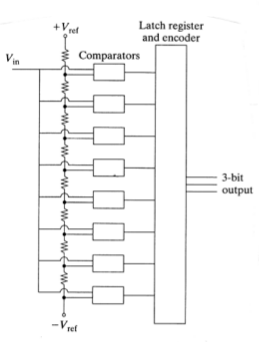
\includegraphics[scale=1]{./Immagini/ADCFlash.png}
\caption{Un ADC flash}
\label{fig:ADCFlash}
\end{center}
\end{figure}
\subsection{L'ADC multipasso}
Si pu\`o ottenere un buon compromesso tra velocit\`a e potenza utilizzando un ADC multipasso.
Questi dispositivi utilizzano dei convertitori ADC flash in cascata e si basano su una serie di scale di espansione:
una serie di moduli sincronizzati suddividono in segnale in modo sempre pi\`u fine al proseguire della digitalizzazione, 
ad esempio il primo modulo digitalizza il segnale su 3 bit, il secondo modulo considera la differenza tra il segnale originale e quello digitalizzato e la ridigitalizza
su una scala pi\`u fine e si procede fino ad una digitalizzazione soddisfacente.\\
Per esempio supponendo di avere in ingresso un segnale da 3.5V il primo ADC potrebbe produrre un segnale digitale corrispondente a 3V, il secondo
si occuperebbe di digitalizzare gli 0.5V rimanenti.\\
Dal punto di vista dell'elettronica, il segnale viene ricevuto e sdoppiato, una parte viene ritardata e l'altra viene digitalizzata, un amplificatore
esegue la differenza tra i segnali e lo manda al modulo successivo, lo schema si trova in figura~\ref{fig:ADCMultipasso}.
\begin{figure}[htbp]
\begin{center}
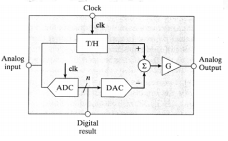
\includegraphics[scale=1]{./Immagini/ADCMultipasso1.png}\\
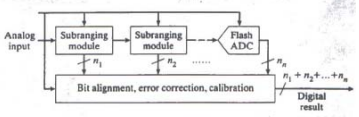
\includegraphics[scale=1]{./Immagini/ADCMultipasso2.png}
\caption{Schema di ADC Multipasso}
\label{fig:ADCMultipasso}
\end{center}
\end{figure}
Questi dispositivi hanno una velocit\`a nell'ordine dalle decine alle centinaia di MHz, ma richiedono una potenza minore (dalle decine a centinaia di mW)
e hanno DNL inferiori (nell'ordine di 0.5 LSB).
\section{Filtraggio e formatura del segnale digitale}
Quando si effettua un filtraggio di un segnale analogico, il segnale in uscita pu\`o essere visto come un integrale di convoluzione
tra la funzione di risposta del filtro e il segnale in ingresso:
\begin{equation*}
V'(t) = \int_{t-L}^t V(t') H(t-t') dt'
\end{equation*}
con $L$ durata del filtro\footnote{\`E interessante interpretare questo integrale come il prodotto di spettri di Fourier del segnale in ingresso e della funzione di risposta del filtro}.\\
Per un segnale digitale, questo integrale diventa una sommatoria:
\begin{equation*}
V'(j) = \sum_{i=j-L}^j V(i)H(j-i)
\end{equation*}
Supponiamo di voler implementare un filtro digitale, un metodo di calcolo della sommatoria \`e dato dal filtro a scorrimento, figura~\ref{fig:filtroScorrimento}.
In questi filtri, ogni passo di sovrapposizione da un $j$ in sequenza.
\begin{figure}[htbp]
\begin{center}
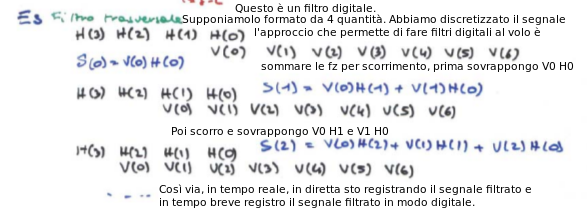
\includegraphics[scale=0.80]{./Immagini/FiltroScorrimento.png}
\caption{Funzionamento matematico di un filtro a scorrimento trasversale}
\label{fig:filtroScorrimento}
\end{center}
\end{figure}
In questo modo il tempo di filtraggio \`e breve e pu\`o essere effettuato in tempo reale, in quanto il segnale filtrato viene calcolato al volo.\\
Utilizzando questa tecnica sul rumore posso fare dei filtri adattivi per rimuoverlo, allo stesso modo \`e possibile realizzare filtri per pile-up facendoli variare
in base al rate.
\section{Analisi della forma dell'impulso}
La forma dell'impulso \`e in grado di contenere informazioni sul tipo di particella incidente, sull'interazione che ha generato l'impulso e sulla posizione spaziale dell'evento.
Queste tipo di elaborazioni sono molto impegnative computazionalmente, per questo devono essere fatte offline (ovvero in un secondo momento) su segnali digitalizzati e memorizzati.
\subsection{Ristabilimento della linea di base}
Se l'impulso viene digitalizzato \`e possibile campionare la linea di base per poter correggere di volta in volta l'impulso;
questa operazione richiede che per un certo lasso di tempo non avvengano eventi, per cui se si vuole campionare il pi\`u possibile
la linea di base per correzioni, \`e necessario trovare un compromesso con il rate di interazioni.
\subsection{Deconvoluzione di impulsi di pile-up}
Se ho un impulso digtalizzato posso utilizzare un programma di analisi degli impulsi per riconoscere ed eseguire la deconvoluzione degli impulsi di pile-up.
Queste operazioni possono essere fatte interpolando i segnali, in quanto dopo la formatura si ha una espressione analitica per interpolare il segnale.
Chiaramente queste operazioni possono essere fatte unicamente offline e con un campionamento molto spinto.
\section{Estrazione di informazioni temporali}
Ci sono misure in cui \`e importante estrarre il momento di arrivo dell'impulso.
La precisione di questa misura dipende dal rivelatore (raccolta delle cariche libere) e dalla catena elettronica (ad esempio range dinamici ampii possono essere problematici).\\
Le \textbf{unit\`a di trigger} si occupano di produrre un impulso logico ogni qual volta venga discriminato un segnale, questi dispositivi sono soggetti a due problemi (figura~\ref{fig:timeJitter}):
\begin{itemize}
\item \textbf{Time jitter}, ogni segnale ha fluttuazioni casuali nel livello e nella forma dell'impulso dovuti, ad esempio, al rumore oppure a tempi diversi di raccolta delle cariche
che portano segnali legati a eventi identici ad avere istanti di trigger diversi. 
Per ridurre questo problema \`e necessario porre il livello di trigger in regioni dove la pendenza \`e massima, per cui \`e meno sensibile a fluttuazioni.
\item \textbf{Amplitude e rise time walk}, la variabilit\`a nel ampiezza massima del segnale (\textit{amplitude walk}) porta ad istanti diversi di trigger,
lo stesso pu\`o accadere per segnali che variano la loro forma. (\textit{time walk}).
Questi problemi si riducono in portata se si abbassa il livello di trigger.
\end{itemize}
\begin{figure}[htbp]
\begin{center}
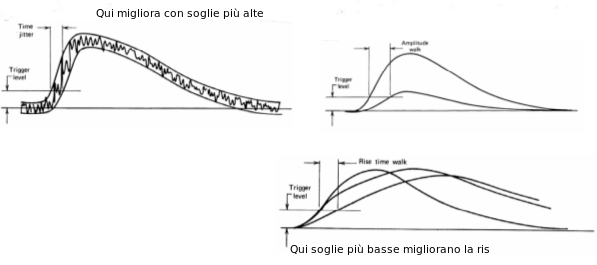
\includegraphics[scale=0.70]{./Immagini/TimeJitter.png}
\caption{Time jitter, amplitude walk e rise time walk}
\label{fig:timeJitter}
\end{center}
\end{figure}
\subsection{Leading edge trigger}
Il leading edge trigger fissa un livello di trigger e produce un impulso logico quanto il segnale supera tale livello, questa tecnica di triggering funziona abbastanza bene se i segnali non hanno un'ampiezza troppo variabile.
Il time jitter ci porta ad alzare il livello di trigger, l'amplitude walk ad abbassarlo: \`e presente un ottimo per soglie intorno al 10-20\% del segnale.
\subsection{Trigger sull'istante di crossover dello zero}
Se un segnale \`e bipolare, l'istante di passaggio del livello zero non \`e dipendente dall'ampiezza dell'impulso.
Per questi segnali \`e possibile eseguire un trigger sul momento del crossover, questa tecnica riesce a risolvere bene il problema dell'amplitude walk,
ma amplifica quello del time jitter.\\
Questa tecnica \`e utilizzabile anche sugli scintilllatori, sottoponendo il segnale anodico ad una singola linea di ritardo, purch\`e la forma
degli impulsi non vari molto.
\subsection{Constant fraction timing}
Se il range dinamico dell'impulso \`e ampio, ci si pu\`o svincolare dall'ampiezza dell'impulso eseguendo il trigger su frazioni $f$ dell'ampiezza massima;
in questo modo, a parit\`a di forma viene risolto il problema dell'amplitude walk.\\
Il constant fraction timing viene effettuato in questo modo (fig~\ref{fig:CFT}):
\begin{enumerate}
\item Il segnale viene sdoppiato
\item Una copia viene invertita e ritardata di un tempo maggiore del tempo di salita
\item L'altra copia viene moltiplicata per un fattore $f$ (quindi attenuata)
\item I segnali vengono sovrapposti e il trigger viene posto sull'istante di zero crossover
\end{enumerate}
\begin{figure}[htbp]
\begin{center}
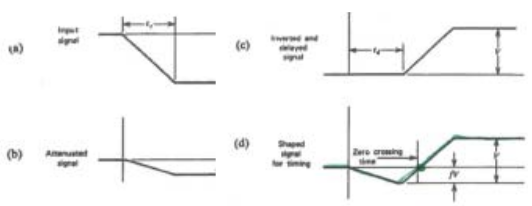
\includegraphics[scale=0.8]{./Immagini/CFT.png}
\caption{Elaborazione di un segnale per il CFT}
\label{fig:CFT}
\end{center}
\end{figure}
Essendo una tecnica basata sul zero crossover, soffre di problemi legati al time jitter, tuttavia risulta un'alternativa migliore in presenza di range dinamici ampii.
\subsection{ARC timing}
L'ARC (Amplitude and Rise time Compensation) timing viene utilizzato in quei rivelatori dove la forma ed il risetime variano, questo accade sopratutto nei rivelatori HPGe.
In questo tipo di timing si suppone che almeno la parte iniziale dell'impulso sia costante e si esegue il trigger sulla parte iniziale dell'impulso.\\
Un sistema ARC esegue queste operazioni(~\ref{fig:ARC}):
\begin{enumerate}
\item Sdoppia il segnale
\item Una copia viene ritardata di un tempo molto inferiore a quello di salita
\item L'altra copia viene invertita ed attenuata
\item I segnali vengono sommati per effettuare un trigger sullo zero crossover
\end{enumerate}
Questo tipo di trigger non compensa l'amplitude walk.
\begin{figure}[htbp]
\begin{center}
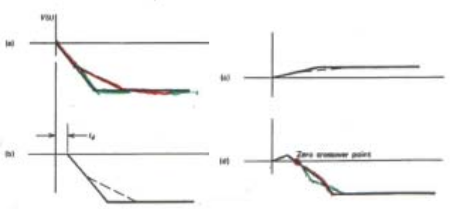
\includegraphics[scale=1]{./Immagini/ARC.png}
\caption{ARC timing}
\label{fig:ARC}
\end{center}
\end{figure}
\subsection{ELET timing}
L'ELET (Extrapolated Leading Edge Trigger) si basa sull'estrapolazione del fronte di salita utilizzando una parte che si suppone essere lineare e costante,
anche questa tecnica viene utilizzata su segnali di forma variabile (sempre HPGe).
Una coppia di discriminatori a soglia con rapporto tra le soglie fissato misurano l'intervallo di tempo tra i due punti ed estrapolano all'indietro il punto di inizio
del segnale.
La misura dell'intervallo di tempo viene effettuata con un TAC (Time to Amplitude Converter).
\subsection{FPET timing}
FPET (First PhotoElectron Trigger) esegue il trigger sul primo fotoelettrone in arrivo, pu\`o essere utilizzato negli scintillatori in condizioni di basso rumore sul fotomoltiplicatore.
\subsection{Confronto dei sistemi di timing}
II LET \`e il migliore per segnali con basso range dinamico e forma costante, il CFT \`e migliore per alti range dinamici e forma costante.
ARC e ELET vengono usati prevalentemente sul HPGe.
\section{Spettroscopia temporale}
\subsection{Spettroscopia temporale con un TAC}
Utilizzando un TAC e un MCA \`e possibile eseguire una spettroscopia temporale, in quanto il TAC produce un impulso proporzionale all'intervallo di tempo.\\
La risoluzione temporale del sistema cos\`i realizzato pu\`o essere misurata sdoppiando e ritardando un segnale che successivamente viene posto in ingresso al TAC.
Un sistema ideale mostrera una larghezza di un bin, nella realta si vedr\`a una regione gaussiana, la cui FWHM sar\`a la risoluzione.\\
Supponiamo di avere una sorgente che emette due quanti in coincidenza rivelati da due dispositivi su due rami diversi, eseguendo una spettroscopia temporale ci\`o che si osserver\`a nell'MCA sar\`a dato dalla sovrapposizione
di due grafici (fig~\ref{fig:spettroCoincidenze}):
\begin{itemize}
\item Un picco centrato in $t_f$ (tempo di ritardo di uno dei due rami) la cui area sar\`a il numero di coincidenze prompt. 
La FWHM indicher\`a la risoluzione del sistema. 
Se i due rami della catena elettronica sono simmetrici, allora il picco osservato sar\`a simmetrico, altrimenti si vedranno asimmetrie.
Ad esempio se il secondo ramo (che fa da stop) ha problemi di amplitude walk, si osserver\`a un'asimmetria verso la coda, in quanto l'amplitude walk ritarder\`a l'arrivo del segnale di stop.
\item Un fondo continuo, dovuto a coincidenze casuali. Se i rate di rivelazione dei due rami, $r_1$ e $r_2$, sono molto inferiori rispetto al reciproco della durata di tempo massima
misurabile dal TAC, allora si osserver\`a un fondo costante di concidenze casuali. \\
Per dimostrarlo calcoliamo la probabilit\`a che si verifichi una coincidenza casuale al tempo $T$.
Supponiamo che ci sia stato un evento nel rivelatore 1, la probabilit\`a che avvenga un evento all'istante $T$ \`e data dalla probabilit\`a
che non avvengano eventi fino al temo $T$ per la probabilit\`a che avvenga un evento tra il tempo $T$ e $T+dT$:
\begin{equation*}
P(T) = e^{-T \, r_2} \, r_2 \, dT
\end{equation*}
Moltiplicando per $r_1$ si ottiene il tasso di coincidenze casuali ad un tempo fissato:
\begin{equation*}
r_{12}=r_1\, r_2 \, e^{-T \, r_2} \, dT
\end{equation*}
Se $r_2\ll T^{-1}$ allora $T\,r_2 \ll 1$ e il termine esponenziale pu\`o essere approssimato a 1 ottenendo:
\begin{equation*}
r_{12} = r_1 \, r_2 \, \Delta T
\end{equation*} 
dove si \`e sostituito $dT$ con $\Delta T$ larghezza di un picco del MCA.
\end{itemize}
\begin{figure}[htbp]
\begin{center}
	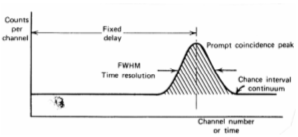
\includegraphics[scale=1]{./Immagini/SpettroCoincidenze.png}
\caption{Analisi con MCA di coincidenze}
\label{fig:spettroCoincidenze}
\end{center}
\end{figure}
Per migliorare il rapporto tra l'area del picco e del fondo si pu\`o migliorare la risoluzione temporale del TAC e introdurre una selezione delle ampiezze.
Avere un'attivit\`a $n$ minore della sorgente pu\`o aiutare dato che le coincidenze casuali vanno come $n^2$ e le reali come $n$.
\subsection{Spettroscopia temporale con un'unit\`a di coincidenza}
Un'unit\`a di coincidenza produce un impulso logico, ogni qualvolta riceve in ingresso due impulsi entro un tempo $\tau$, esso rappresenta, quindi, una sorta di SCA sul tempo.\\
Questo dispositivo, insieme ad un dispositivo per produrre ritardi variabili, pu\`o essere usato per eseguire spettroscopie temporali.
Riprendendo il sistema a due rivelatori precedente, sottoponiamo un segnale ad un ritardo fissato $t_f$ e l'altro ad un ritardo variabile $t_v$.
Se $\tau = \frac {\Delta T} { 2}$ (l'intervallo registrato \`e $(-\tau , +\tau)$) allora l'unit\`a di coincidenza esegue lo stesso numero di conteggi di un canale dell'MCA:
variando $t_v$, l'unit\`a segnaler\`a le coincidenze temporali con tempo $t_f - t_v$.\\
In questi sistemi \`e importante impostare bene $\tau$, se esso \`e troppo grande esso contegger\`a troppe coincidenze casuali, se \`e troppo piccolo sar\`a difficile vedere
il picco delle coincidenze casuali. 
Il valore migliore risulta $\tau = L/2$ con $L$ larghezza alla base del picco, scegliere dei $\tau$ sopra questa media porter\`a a dei plateau di coincidenze casuali (fig.~\ref{fig:plateau}),
andare sotto ridurr\`a l'altezza del picco, rendendolo pi\`u difficile da individuare.
\begin{figure}[htbp]
\begin{center}
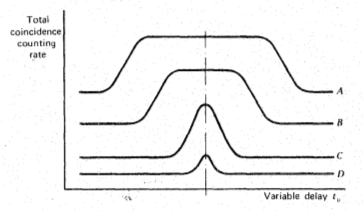
\includegraphics[scale=1]{./Immagini/Plateau.png}
\caption{Esempi di spettri ottenuti con questa tecnica al variare di $\tau$}
\label{fig:plateau}
\end{center}
\end{figure}
Normalmente non si prende il valore minimo di $\tau$, in quanto possono capitare derive temporali che modificano il rate di eventi;
per questo esso viene preso un po' pi\`u grande del minimo.
\subsection{Correzione delle coincidenze casuali}
Nel caso di coincidenze casuali a due la correzione del fondo \`e piuttosto semplice in quanto esso \`e piatto e vale $2 \tau \, r_1 \, r_2$.\\
La situazione diventa pi\`u complicata per le coincidenze multiple, per esempio per le coincidenze a tre esiste un fondo piatto $2 \tau  \, r_1 \, r_2$,
tuttavia esiste anche la possibilit\`a di avere una coincidenza reale a due con una casuale. 
Quest'ultima \`e difficilmente valutabile e spesso si ricorre ad un'analisi sperimentale per determinare il fondo.
\subsection{Determinazione di $\tau$}
Il fondo delle coincidenze a due pu\`o essere utilizzato per determinare $tau$ usando, ad esempio, due sorgenti scorrelate ben schermate oppure utilizzando
una sola sorgente che emetta quanti non in coincidenza.\\
Un'altra possibilit\`a pu\`o venire dal misurare la larghezza del plateau, in questo caso \`e utile una sorgente che emetta un'elevata quantit\`a di 
radiazione in coincidenza.
\subsection{Misura di coincidenze ritardate}
Supponiamo di avere una sorgente che emetta due quanti in sequenza passando per uno stato metastabile a vita media inferiore alla risoluzione temporale del sistema.
In questo caso vedremo un picco gaussiano di coincidenze vere con una coda sulla destra di tipo esponenziale, da essa si pu\`o estrarre le informazioni di interesse sulla vita dello stato.\\
Questa misura pu\`o essere effettuata utilizzando un MCA, oppure utilizzando un'unit\`a di coincidenza che effettui una scansione della regione di interesse.\\
Un'altra di questo tipo viene effettuata con la spettroscopia T.O.F. di neutroni, misurando l'intervallo di tempo tra l'istante di produzione e di arrivo
dei neutroni ad un rivelatore, si pu\`o misurare la loro energia.
\subsection{Misure di attivit\`a}
Supponiamo di avere una sorgente che emette 2 quanti $q_1$ e $q_2$ di radiazione in coincidenza con attivit\`a $S$ senza alcuna correlazione angolare, inoltre immaginiamo di avere un rivelatore
sensibile solo ai quanti di tipo $q_1$ e un altro rivelatore sensibile solo ai quanti di tipo $q_2$.\\
Siano $\epsilon_1$ e $\epsilon_2$ le relative efficienze (comprensive di fattori angolari, di efficienze di interazione e altro), allora i tassi di rivelazione saranno:
\begin{gather}
r_1 = \epsilon_1 \, S\\
r_2 = \epsilon_2 \, S
\end{gather}
mentre il tasso di coincidenze vere rivelate sar\`a:
\begin{equation*}
r_{t} = \epsilon_1 \, \epsilon_2 \, S
\end{equation*}
Chiamando $r_{ch}$ il tasso di coincidenze casuali, allora il tasso di coincidenze totali misurate sar\`a
$r_{12} = r_{t} + r_{ch} = \epsilon_1 \, \epsilon_2 \, S + r_{ch} $, risolvendo il sistema si trova:
\begin{equation*}
S = \frac{r_1 \, r_2}{r_{12}-r_{ch}}
\end{equation*}
ovvero l'attivit\`a della sorgente.\\
Questo questo metodo si pu\`o misurare con una accuratezza del 1\% le attivit\`a delle sorgenti senza avere rivelatori che coprano l'intero angolo solido;
inoltre se un rivelatore copre l'angolo solido, allora si pu\`o rinunciare al bisogno di avere radiazione scorrelata angolarmente.\\
Questo metodo tipicamente viene applicato su coincidenze $\beta-\gamma$.
Un rivelatore sensibile solo ai $\gamma$ pu\`o essere ottenuto interponendo un assorbitore di $\beta$ prima del rivelatore, tuttavia un rivelatore
sensibile ai $\beta$ misura sempre qualche fotone, in questo caso \`e necessario cercare di selezionare le energie.\\
Coincidenze $\gamma - \gamma$ sono ancora pi\`u difficili, in quanto anche selezionando le energie, il fondo per l'effetto Compton da sempre parecchi problemi.
\section{Moduli per misure temporali}
\subsection{Moduli di trigger}
I moduli di trigger andrebbero posti subito dopo il rivelatore, tuttavia questo comporta un peggioramento della FWHM.\\
Per questo se si \`e interessati a mantenere l'informazione sull'energia \`e meglio metterlo dopo lo stadio di preamplificazione, dove,
se la salita dell'impulso \`e veloce, l'informazione temporale viene preservata.\\
L'eccezione viene dagli scintillatori, dove, utilizzando una resistenza di carico da 50 $\Omega$ (che genera segnali pi\`u veloci), il segnale all'anodo pu\`o essere utilizzato per misure temporali, 
mentre utilizzando una resistenza pi\`u grande tra l'ultimo dinodo e l'anodo si pu\`o ottenere un segnale a coda lunga con informazioni sull'energia.\\
Altri moduli di trigger possono richiedere una formatura (ad esempio lo zero crossover), in questo caso vanno posti dopo l'amplificatore,
talvolta i moduli di trigger sono integrati in discriminatori o SCA, in modo da non sacrificare troppo l'informazioni sull'ampiezza.
\subsection{Unit\`a di coincidenza}
Se si \`e interessati ad una misura di sovrapposizione degli impulsi, allora il $\tau$ di coincidenza deve essere pari alla larghezza dell'impulso, mentre
se il circuito \`e sensibile al fronte di salita dell'impulso, allora il $\tau$ pu\`o essere scelto liberamente in base alle necessit\`a.\\
Spesso questi dispositivi possiedono pi\`u ingressi (da 1 a 4) che possono essere attivati o disattivati a seconda delle necessit\`a (concidenze a 2, a 3,...);
uno di questi ingressi a volte funge da anticoincidenza, per inibire il dispositivo quando necessario.
\subsection{TAC}
Questo dispositivo viene utilizzato insieme ad un MCA e produce un segnale lineare proporzionale all'intervallo di tempo tra due segnali di start e stop.
In questi dispositivi \`e fondamentale la linearit\`a, essa pu\`o essere misurata sdoppiando segnali e sottoponendoli a linee di ritardo.\\
Esistono TAC di due tipi:
\begin{itemize}
\item \textbf{A sovrapposizione}, il TAC riceve in ingresso due impulsi logici standard e misura l'area di sovrapposizione dei due segnali di start e stop.
Se essi sono in perfetta coincidenza allora gli impulsi si sovrapporranno perfettamente, altrimenti l'area sar\`a proporzionale all'intervallo di tempo: un integratore misura quest'area e d\`a l'informazione.
Questi dispositivi sono veloci nella misura, ma hanno problemi di linearit\`a e precisione, per cui vengono utilizzati in caso di alti rate.
\item \textbf{A start-stop}, in questi dispositivi i segnali di start e stop iniziano e interrompono l'accumulo di carica a corrente costante su un condensatore.
In questo modo la tensione ai capi sar\`a linearmente proporzionale al tempo, ottenendo un'ottima linearit\`a.
\end{itemize}
\subsection{TDC, Time to Digital Converter}
Non \`e molto sensato dover produrre un impulso lineare per poi digitalizzarlo, per questo esistono dispositivi che producono direttamente impulsi digitali.
In questi moduli viene prodotta un gate della durata dell'intervallo, questo gate controlla l'uscita di impulsi di clock a frequenza costante.\\
La frequenza massima attuale \`e di 1 GHz, per cui si pu\`o avere una precisione massima di 1 ns. 
Questo risulta problematico per impulsi brevi (a 20 ns, l'errore \`e del 5\%), per questo spesso i TDC sono corredati con dilatatori di impulsi
che interpolano e dilatano l'impulso temporale.
\subsection{Sistemi di ritardo}
Utilizzando cavi coassiali di diversa lunghezza \`e possibile realizzare sistemi di ritardo nella scala dei ns, tuttavia sopra i 100 ns questo sistema non \`e utilizzabile.
Per ritardi nei $\mu$s si possono utilizzare cavi coassiali con materiali speciali, tuttavia devono essere usati solo per portare segnali a bassa frequenza,
in quanto i segnali ad alta frequenza vengono fortemente distorti.
Spesso questi sistemi sono integrati in amplificatori per mettere a punto sistemi basati sulla temporizzazione.\\
Per ritardare gli impulsi logici poich\`e non si ha informazioni contenute nella forma si possono usare altri sistemi.
Uno di questi \`e basato sulla discriminazione di una rampa: l'impulso da ritardare avvia la salita di una rampa, quando essa supera un livello di discriminazione
viene prodotto un segnale logico in uscita, variando il livello si possono ottenere i ritardi desiderati.
\subsection{Amplificatori a banda larga e filtri temporali}
Talvolta pu\`o essere fondamentale mantenere l'informazione temporale, in questi casi \`e utile riuscire a mantenere il segnale inalterato nella forma
dopo lo stadio di amplificazione.
Un amplificatore a banda larga esegue questa operazione, amplifica semplicemente il segnale senza effettuare alcuna formatura.
Questo modulo \`e utile ad esempio con l'uscita anodica di un fotomoltiplicatore.\\
Se invece si necessita di una formatura minimale, allora si pu\'o utilizzare un filtro temporale, esso esegue un formatura con tempi
caratteristici inferiori ai comuni amplificatori, mantenendo cos\`i inalterata l'informazione temporale a costo di un rapporto segnale-rumore peggiore.
\section{Pulse Shape Discrimination e Rise Time Discrimination}
La forma dell'impulso \`e in grado di contenere informazioni come il tipo di particella che ha interagito con il rivelatore oppure la raccolta delle cariche.
Queste informazioni possono essere ottenute attraverso la PSD o la RTD.
La prima risulta efficace su segnali lineari veloci (come gli impulsi anodici), la seconda \`e equivalente alla PSD sugli impulsi lenti, come quelli del PRE.\\
La PSD pu\`o essere utile in questi casi:
\begin{itemize}
\item	Discriminazione del fondo $\gamma$ negli scintillatori organici se usati come rivelatori di neutroni veloci
\item Riconoscimento del tipo di particella in alcuni scintillatori inorganici
\item Discriminazione tra particelle a range breve e lungo nei contatori proporzionali (tipo le camere a gas)
\item Eliminazione di impulsi spuri nel Ge e nel Si
\item Reiezione di pile-up, osservando le deformazioni
\end{itemize}
Esistono due approcci possibili, uno \`e basato sul sentire le differenze nel rise time, l'altro \`e basato sull'integrazione del segnale in diversi punti:
\begin{itemize}
\item Con due discriminatori a soglie fissate si possono produrre segnali di start e stop per un TAC e osservare la velocit\`a del fronte di salita
\item Si pu\`o rendere il segnale bipolare e poi utilizzare un crossover. 
L'istante di crossover non dipende dall'ampiezza, bens\`i solo dalla forma, per cui misurando l'intervallo di tempo tra un punto fissato (ad esempio il 10\% del fronte di salita)
e lo zero crossover con un TAC ed eseguendo la spettroscopia con un MCA si pu\`o determinare il tipo di particella (fig~\ref{fig:PSD}). 
Un SCA pu\`o essere utilizzato per selezionare il tipo di particella di interesse.
\item Si pu\`o integrare il segnale in due istanti diversi ed eseguire il rapporto dell'integrazione. Questo rapporto non dipende dall'ampiezza e da un
fattore di discriminazione della forma.
\end{itemize}
Si introduce la figura di merito:
\begin{equation*}
M = \frac{X}{W_a + W_b}
\end{equation*}
questo fattore da una misura della qualit\`a della separazione dei segnali ottenuta con il PSD, esso dipende dal range dinamico dei segnali,
per la definizione di $X$, $W_a$ e $W_b$ vedere figura~\ref{fig:PSD}.
\begin{figure}[htbp]
\begin{center}
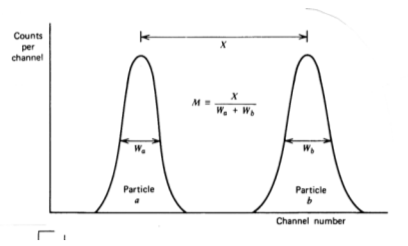
\includegraphics[scale=1]{./Immagini/PSD.png}
\caption{PSD con zero crossover e figura di merito}
\label{fig:PSD}
\end{center}
\end{figure}